\documentclass[10pt,-letter paper]{article}
\usepackage[left=1in, right=0.75in, top=1in, bottom=0.75in]{geometry}
\usepackage{graphicx} % Required for inserting images
\usepackage{siunitx}
\usepackage{setspace}
\usepackage{gensymb}
\usepackage{xcolor}
\usepackage{caption}
%\usepackage{subcaption}
\doublespacing
\singlespacing
\usepackage[none]{hyphenat}
\usepackage{amssymb}
\usepackage{relsize}
\usepackage[cmex10]{amsmath}
\usepackage{mathtools}
\usepackage{amsmath}
\usepackage{commath}
\usepackage{amsthm}
\interdisplaylinepenalty=2500
%\savesymbol{iint}
\usepackage{txfonts}
%\restoresymbol{TXF}{iint}
\usepackage{wasysym}
\usepackage{amsthm}
\usepackage{mathrsfs}
\usepackage{txfonts}
\let\vec\mathbf{}
\usepackage{stfloats}
\usepackage{float}
\usepackage{cite}
\usepackage{cases}
\usepackage{subfig}
%\usepackage{xtab}
\usepackage{longtable}
\usepackage{multirow}
%\usepackage{algorithm}
\usepackage{amssymb}
%\usepackage{algpseudocode}
\usepackage{enumitem}
\usepackage{mathtools}
%\usepackage{eenrc}
%\usepackage[framemethod=tikz]{mdframed}
\usepackage{listings}
%\usepackage{listings}
\usepackage[latin1]{inputenc}
%%\usepackage{color}{   
%%\usepackage{lscape}
\usepackage{textcomp}
\usepackage{titling}
\usepackage{hyperref}
%\usepackage{fulbigskip}   
\usepackage{tikz}
\usepackage{graphicx}
\lstset{frame=single,breaklines=true}
\let\vec\mathbf{}
\usepackage{enumitem}
\usepackage{graphicx}
\usepackage{siunitx}
\let\vec\mathbf{}
\usepackage{enumitem}
\usepackage{graphicx}
\usepackage{enumitem}
\usepackage{tfrupee}
\usepackage{amsmath}
\usepackage{amssymb}
\usepackage{mwe} % for blindtext and example-image-a in example
\usepackage{wrapfig}
\graphicspath{{figs/}}
\providecommand{\cbrak}[1]{\ensuremath{\left\{#1\right\}}}
\providecommand{\brak}[1]{\ensuremath{\left(#1\right)}}
\newcommand{\sgn}{\mathop{\mathrm{sgn}}}
\providecommand{\abs}[1]{\left\vert#1\right\vert}
\providecommand{\res}[1]{\Res\displaylimits_{#1}} 
\providecommand{\norm}[1]{\left\lVert#1\right\rVert}
%\providecommand{\norm}[1]{\lVert#1\rVert}
\providecommand{\mtx}[1]{\mathbf{#1}}
\providecommand{\mean}[1]{E\left[ #1 \right]}
\providecommand{\fourier}{\overset{\mathcal{F}}{ \rightleftharpoons}}
%\providecommand{\hilbert}{\overset{\mathcal{H}}{ \rightleftharpoons}}
\providecommand{\system}{\overset{\mathcal{H}}{ \longleftrightarrow}}
%\newcommand{\solution}[2]{\textbf{Solution:}{#1}}
%\newcommand{\solution}{\noindent \textbf{Solution: }}
\newcommand{\cosec}{\,\text{cosec}\,}
\providecommand{\dec}[2]{\ensuremath{\overset{#1}{\underset{#2}{\gtrless}}}}
\newcommand{\myvec}[1]{\ensuremath{\begin{pmatrix}#1\end{pmatrix}}}
\newcommand{\myaugvec}[2]{\ensuremath{\begin{amatrix}{#1}#2\end{amatrix}}}
\newcommand{\mydet}[1]{\ensuremath{\begin{vmatrix}#1\end{vmatrix}}}

\begin{document}

\author{SUJAL GUPTA$^{*}$ FWC22259}
\title{CBSE Class 10, 2013}

\maketitle

\bigskip


\begin{enumerate}
\section{Algebra}
\item The common difference of the AP $\frac{1}{p}$,$\frac{1-p}{p}$,$\frac{1-2p}{p}$..... is :
 \begin{enumerate}
    \item p\\
    \item -p\\
    \item -1\\
    \item 1 \\
 \end{enumerate}
 \item Solve the following quadratic equation for $x$ :\\ $4\sqrt{3}x^2+5x-2\sqrt{3}=0$
\item How many three-digit natural numbers are divisible by 7?
\item For what value of $k$, are the roots of the quadratic equation $kx (x-2) + 6 = 0$ equal ?
\item Find the numbers of terms of the AP $18$,$15\frac{1}{2}$,$13$,....,$-49\frac{1}{2}$ and find the sum of all its terms.
\item Solve the following for $x$ : \\
$\frac{1}{2a+b+2x}=\frac{1}{2a}+\frac{1}{b}+\frac{1}{2x}$ \\
\item If the sum of first 7 terms of an AP is 49 and that of first 17 terms is 289, find the sum of its first $n$ terms. 
 \section{Geometry}
\item In \figref{fig:fig1}, PA and PB are two tangents drawn from an external point P to a
circle with centre C and radius 4 cm. If PA $\perp$ PB, then the length of each
tangent is :
\begin{figure}[H]
			\centering
			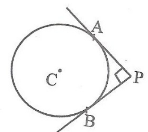
\includegraphics[width=\columnwidth]{1.png}
\caption{tangent PA and PB}
    \label{fig:fig1}
		\end{figure}
 \begin{enumerate}
    \item 3 cm\\
    \item 4 cm\\
    \item 5 cm\\
    \item 6 cm
 \end{enumerate}
\item In \figref{fig:fig2}, a circle with centre O is inscribed in a quadrilateral ABCD such
that, it touches the sides BC, AB, AD and CD at points P, Q, R and S respectively. If AB=29 cm, AD=23 cm, $\angle$B=90$\degree$ and DS = 5 cm, then the radius of the circle (in cm.) is : \\
		\begin{figure}
			\centering
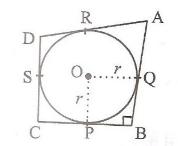
\includegraphics[width=0.5\columnwidth]{2.png}
\caption{Quadrialteral ABCD}
\label{fig:fig2}
		\end{figure}
 \begin{enumerate}
    \item 11\\
    \item 18\\
    \item 6\\
    \item 15
 \end{enumerate}
 \item In \figref{fig:fig3}, the area of triangle ABC in sq. units) is :
	\begin{figure}[H]
		\centering
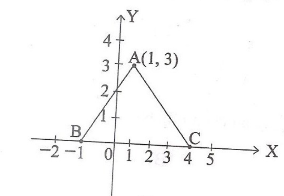
\includegraphics[width=\columnwidth]{3.png}
\caption{Triangle ABC}
\label{fig:fig3}
	\end{figure}
 \begin{enumerate}
    \item 15\\
    \item 10\\
    \item 7.5\\
    \item 2.5
 \end{enumerate}
 \item If the difference between the circumference and the radius of a circle is 37 cm, then using $\pi=\frac{22}{7}$, the circumference (in cm) of the circle is:
 \begin{enumerate}
    \item 154\\
    \item 44\\
    \item 14\\
    \item 7
 \end{enumerate}
 \item In \figref{fig:fig4}, a circle inscribed in triangle ABC touches its sides AB, BC and AC at points D, E and F respectively. If AB = 12 cm, BC = 8 cm and AC = 10 cm, then find the lengths of AD, BE and CF.
	\begin{figure}[H]
		\centering
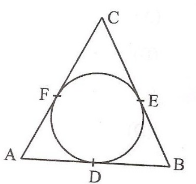
\includegraphics[width=\columnwidth]{4.png}
\caption{Circle in Triangle ABC}
\label{fig:fig4}
\end{figure}
\item Prove that the parallelogram circumscribing a circle is a rhombus.
\item Two circular pieces of equal radii and maximum area, touching each other are cut out from a rectangular card board of dimensions 14 cm$\times$7 cm. Find the area of the remaining card board. $\brak{ \pi = \frac{22}{7}}$
\item A vessel is in the form of a hemispherical bowl surmounted by a hollow cylinder of same diameter. The diameter of the hemispherical bowl is 14 cm and the total height of the vessel is 13 cm. Find the total surface area of the vessel. $\brak{ \pi = \frac{22}{7}}$
\item A wooden toy was made by scooping out a hemisphere of same radius from each end of a solid cylinder. If the height of the cylinder is 10 cm,  and its base is of radius 3.5 cm, find the volume of wood in the toy. $\brak{ \pi = \frac{22}{7}}$
\item In a circle of radius 21 cm, an arc subtends an angle of 60$\degree$ at the centre. Find :  \begin{enumerate} 
\item the length of the arc
\item area of the sector formed by the arc.[Use $\pi = \frac{22}{7}$]
\end{enumerate}
\item Sum of the areas of two squares is 400 cm$^2$. If the difference of their perimeters is 16 cm, find the sides of the two squares.

\item Prove that the tangent at any point of a circle is perpendicular to the radius through the point of contact.


\item In \figref{fig:fig5}, $l$ and $m$ are two parallel tangents to a circle with centre O, touching the circle at A and B respectively. Another tangent at C intersects the line $l$ at D and $m$ at E. Prove that $\angle$ DOE = 90$\degree$.
\begin{figure}[H]
\centering
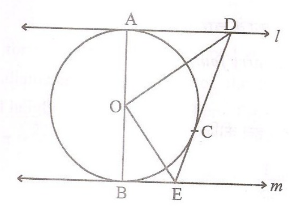
\includegraphics[width=\columnwidth]{5.png}
\caption{Tangents touching circle at A and B}
\label{fig:fig5}
 \end{figure}

 \item Water is flowing through a cylindrical pipe, of internal diameter 2 cm, into a cylindrical tank of base radius 40 cm, at the rate of 0.4 m/s. Determine the rise in level of water in the tank in half an hour.
\item A bucket open at the top, and made up of a metal sheet is in the form of a frustum of a cone. The depth of the bucket is 24 cm and the diameters of its upper and lower circular ends are 30 cm and 10 cm respectively. Find the cost of metal sheet used in it at the rate of Rs 10 per 100 cm$^2$.$\brak{ \pi = \frac{22}{7}}$
  \section{Trigonometry}
\item The angle of depression of a car, standing on the ground, from the top of a
75 m high tower, is 30$\degree$. The distance of the car from the base of the tower
(in m.) is : \\
 \begin{enumerate}
    \item 25$\sqrt{3}$\\
    \item 50$\sqrt{3}$\\
    \item 75$\sqrt{3}$\\
    \item 150
 \end{enumerate}
 \item The horizontal distance between two poles is 15 m. The angle of depression of the top of first pole as seen from the top of second pole is 30$\degree$. If the height of the second pole is 24 m, find the height of the first pole. $\brak{ \pi = \frac{22}{7}}$
 
\item The angle of elevation of the top of a building from the foot of the tower is 30$\degree$ and the angle of elevation of the top of the tower from the foot of the building is 60$\degree$. If the tower is 60 m high, find the height of the building. 
  \section{Probability}
\item  The probability of getting an even number, when a die is thrown once, is :

 \begin{enumerate}
    \item $\frac{1}{2}$\\
    \item $\frac{1}{3}$\\
    \item $\frac{1}{6}$\\
    \item $\frac{5}{6}$
 \end{enumerate}
 \item A box contains 90 discs, numbered from 1 to 90. If one disc is drawn at random from the box, the probability that it bears a prime-number less than 23 is :
 
 \begin{enumerate}
    \item $\frac{7}{90}$\\
    \item $\frac{10}{90}$\\
    \item $\frac{4}{45}$\\
    \item $\frac{9}{89}$
 \end{enumerate}


\item A card is drawn at random from a well shuffled pack of 52 playing cards. Find the probability that the drawn card is neither a king nor a queen.

\item A group consists of 12 persons, of which 3 are extremely patient, other 6 are extremely honest and rest are extremely kind. A person from the group is selected at random. Assuming that each person who is (i) extremely patient (ii) extremely kind or honesty. Which of the above values you prefer more.
 \section{Construction}
\item Construct a triangle with sides 5 cm, 4 cm and 6 cm. Then construct another triangle whose sides are $\frac{2}{3}$ times the corresponding sides of first triangle.

\item In \figref{fig:fig6}, AB and CD are two diameters of a circle with centre O, which are perpendicular to each other. OB is the diameter of the smaller circle. If OA =7 cm, find the area of shaded region .$\brak{ \pi = \frac{22}{7}}$\\
	\begin{figure}[H]
		\centering
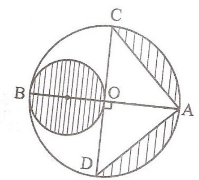
\includegraphics[width=\columnwidth]{6.png}
\caption{AB and CD diameters of circle}
\label{fig:fig6}
	\end{figure}
\section{Coordinate Geometry}
\item Prove that the points $(7, 10), (-2, 5) $and $(3, -4)$ are the vertices of an isosceles right triangle.
\item Find the ratio in which the $y$-axis divides the line segment joining the points $(-4,-6)$ and $(10,12)$. Also find the coordinates of the point of division.


\item The three vertices of a parallelogram $ABCD$ are $\vec{A}(3, -4)$, $\vec{B}(-1, -3)$ and $\vec{C}(-6, 2)$. Find the coordinates of vertex $\vec{D}$ and find the area of $ABCD$.
\setcounter{figure}{1}
\end{enumerate}
\end{document}
